\documentclass[UTF8]{ctexart}
\usepackage{underscore}
\usepackage{graphicx}
\title{周报}
\author{LiuYan}
\date{\today}
\begin{document}

\tableofcontents
\maketitle
\section{2018.8.28}
\subsection{练习相关git命令:}
rm -f file 删除文件\\
git reset --hard $HEAD^{\Lambda}$  丢弃本次的修改\\
ctrl+C 杀死当前进程\\
git reset --hard ID号  后悔删除了添加又加回来\\
nautilus显示当前目录窗口\\
git diff HEAD -- file.txt  查看不同\\
git reset HEAD file1.txt 撤销ADD\\
git remote add origin git@github.com:iMurphL/report.git\\
git push -u origin master 把本地库的版本推送到远程库中\\
git clone git@github.com:iMurphL/report.git 从远程库克隆到本地库\\
\subsection{念书subpaving}
念完啦《applied interval analysis》第三章subpaving,这里介绍了两种算法:直接映射和逆运算的subpaving算法。相比于一般的subpaving,有规则的subpaving更加易于操作和结果的存储,但是他需要花费巨大的存储空间,因此只适用于低维度的计算。对于高维度的问题,他将介绍新的方法:紧缩方法.\\
\subsection{实践git}
尝试用自己的github帐号建了一个远程库,并实现了分布版本管理。
\subsection{linux}
在windows上装了虚拟机和ubuntu.

\section{2018.8.29}
\subsection{上午新生见面会}
\subsection{下午政治课}
毛中特第二节课,讲述了空想社会主义和共产党宣言。\\

自然辩证法第二节课,讲述了古代唯物观的发展历程。\\

\section{2018.8.30}
\subsection{念书contractors}
在看《applied interval analysis》第四章contractors,暂时称其为紧缩方法吧。它就是找到一个更小的阈来代替原有的X,并且以解集不变为前提。刚看完高斯消除和高斯赛德方法。
\subsection{git}
管理和创建分支:\\
git checkout -b dev 创建并切换到分支dev上\\
解决冲突\\
解决冲突是在分支和主线上同时存在修改提交时产生冲突时的应对方法\\
git merge --no-ff -m "merge with no-ff" dev 解决fast forward模式没有分支信息的困扰\\
git stash 储存当前工作现场,与中断相似\\
git stash apply恢复到当前工作现场 git stash drop删除stash内容\\
git stash pop 恢复工作现场并删除stash内容\\
git stash list 查看stash内容\\
git stash apply stash@{0}恢复指定的stash现场\\
git remote -v 查看远程库的信息\\
git branch -D dev origin/dev 创建本地分支\\
git branch lianjie 设置链接\\
git pull 从远程库抓取分支\\
git rebase 解决多人协作的冲突\\
git tag v1.0 创建标签\\
git tag v0.9 ID号 给过去的ID号打标签\\
git show v0.9 查看标签信息\\
git tag -a v1.0 -m "message" ID号  指定标签信息\\
git pushi origin v1.0 推送一个本地标签\\
git push origin --tags 推送全部未推送过的本地标签\\
git push origin :refs/tags/v1/0 删除一个远程标签\\
ssh -l liuyan IP号 连接到另一个服务器\\

\section{2018.8.31}
\subsection{银行卡}
上午去建设银行排队激活银行卡
\subsection{生产实习}
下午指导本科生焊板子:刮锡(注意刮板要和钢网成45度角)~贴片机(注意校准,先单步运行再高速运行)~手动摆件~高温回流焊~手焊\\
\subsection{Latex}
晚上去国内的CTEX网站下载了包括Miktex的镜像文件,网址是:\\
http://www.ctex.org/CTeXDownload

下载完成后打开winedit按照教程编辑日志,输入文本后保存并把文件格式更改为UTF-8,在编译输出pdflatex文件,结果是一堆乱码。\\

我试着从简单的公式开始编辑,下面是公式表示方法链接,发现可以输出比较好看的pdf。那么编辑器是没有问题的,我把文件格式改成了默认的tex格式结果还是没有用。\\
http://blog.sina.com.cn/s/blog5e16f1770100fs38.html\\

通过百度对比之后发现带中文的编辑和英文编辑的模板是不一样的,于是解决了这个问题:\\
https://blog.csdn.net/lkj345/article/details/50516685\\
https://blog.csdn.net/pipisorry/article/details/54571521\\
\section{2018.9.1}
\subsection{写日志时遇见的一些问题}
1.写完一天的日志后运行错误,仔细排查发现文件格式保存错误,应该是UTF-8格式而不是tex.\\

2.重新打开之前的文件不能显示,提示read error.我新建文件,把文档重新从notepad++上复制过来保存运行才可以了。\\

3.我发现每次写一堆东西之后导出pdf会有一堆错误但是不知道在哪改,改起来摸不着头脑花了好长时间,所以现在基本上写一点就导出一点很方便吖\\

4.想要去除日期前面的段的序号,只要在段命令里添个*即可啦。
\section{2018.9.2}
\subsection{师兄的福利}
师兄给传了一个ubuntu的驱动过来,先存在windows D盘文件夹。
\subsection{notepad++}
安装notepad++,方便打草稿,新建my file文件夹用来装文档。
\section{2018.9.3}
\subsection{重装ibex}
安装虚拟机,在虚拟机上装ubuntu.打开终端进入root用户权限:su root ,失败提示:su:Authentication failure.\\
百度解决方法:这是因为首次进入需要用户激活密码,命令如下:\\
sudo passwd\\
然后系统会提示你输入要设置的密码两遍就好了。\\

在安装gcc时系统提示:Could not get lock /var/lib/dpkg/lock - open (11: Resource temporarily unavailable)\\
百度解决方法:因为有别的apt进程在进行,需要杀死之前apt进程。命令如下:\\
sudo rm /var/lib/dpkg/lock\\
sudo dpkg --configure -a\\

写了一个简单的区间运算程序可以运行,但是上次的程序依然提示两处错误。一处是没有声明f函数,另一处是在函数库里没有DIFF这个函数。于是程序加了一行Function f(x,sin(x)+1)之后解决了第一处错误,但是系统依然显示另一处: error: ‘class ibex::Function’ has no member named ‘eval_affine’\\
 Interval z=df.eval_affine(x); \\
 
makefile文件的作用:告诉系统ibex头文件的位置。如果没有makefile可用以下命令代替:\\
pkg-config --cflags ibex    (找出路径)\\
g++ -I/usr/local/include -I/usr/local/include/ibex -I/usr/local/include/ibex/3rd lab1.cpp -o lab1
./lab1\\
\subsection{Latex}
发现一篇新的教程如下,可以用Texmaker+Ctex来做Latex排版。发现texmaker比winedit好用很多,以后就不用winedit了。\\
https://blog.csdn.net/tingzuhuitou/article/details/77539887\\
\subsection{机械臂}
用vs2013+opencv能识别特定颜色和进行边缘化\\
\subsection{智能分析方法:}
数值迭代法:流程图,三种终止准则\\
线性规划linear programming:标准数学模型(矩阵形式),可行解与可行域\\
作业:从互联网搜索一些可信度高的线性规划工具箱和开源代码。\\
\section{2018.9.4}
\subsection{线性规划}
本想查找线性规划资料,在github上找到了一些网站的源代码,就想着可以试着用sphinx生成静态html看一看吖\\

更新pip:本想用pip命令安装sphinx,cmd窗口提示我在用pip10.0但是电脑里有pip18.0,发生了冲突。这是因为安装了多个版本的python.需要卸载一些。\\
卸载了所有的python只留下一个python3.7的安装包,并安装它\\
打开命令窗口,按照官网教程安装pip,https://pip.pypa.io/en/stable/installing/\\

pip安装好了就可以用pip install sphinx安装sphinx了。\\

sphinx-quickstart回答问题会在根目录生成文件conf.py和index.rst,把这两个文件和makefile放在同一个文件夹比如LiuYan下,然后sphinx-build -b html LiuYan/ _build/在根目录下就会生成包含
html的_build文件夹啦。\\

找资料的时候又找到了生成html的ipynb文件,百度发现安装jupyter notebook就可以看啦。资料文件位置:/D:/线性规划  \\

找到一个线性规划工具包:pulp\\
安装过程:https://pythonhosted.org/PuLP/main/installing_pulp_at_home.html
$\#$
installation\\

通过pulp在命令窗口切换到Python命令行优化了两个实际问题:汽车生产资源分配问题和制作火腿原料混合比例问题。\\
\subsection{note}
解决电脑里python3.7和anaconda中python3.6的共存冲突问题。注意:\\
python3.7里的pip会把所有的东西安装到它的lib文件夹下,所以和anaconda的pip是不一样的要注意。\\

总结:1.通过查阅网络资料发现,anaconda自带sphin,jupyter notebook,只要把它们的路径加到环境变量中即可使用。\\
     2.一定不要妄想一个软件的两个版本能共存,很容易冲突和出错,所以我卸载了python3.7,以后就用anaconda+pycharm.\\ \subsection{cmake}
cmake:cross platform make的缩写,是个可以跨平台的编译工具,它可以输出makefile文件和c++文件.而且它不会完全建构出最终的软件,而是产生稳定的建构档,方便程序员建构他的软件。\\
这里说的建构软件源于建筑学,是指建筑起软件结构。\\
软件结构(Software Structure)是指一种层次表况,由软件组成成分构造软件的过程、方法和表示。软件结构主要包括程序结构和文档结构。程序结构有两层含义,
一是指程序的数据结构和控制结构;另一是指由比程序低一级的程序单位(模块)组成程序的过程、方法和表示。在后者含义下,具有代表性的是块结构和嵌套结构两种。
块结构比较自然,各个部分之间通过一些公用变量取得联系,嵌套结构是在嵌套分程序的基础上引进局部性和动态性,以减少程序的初始信息量,嵌套结构不如块结构直观,调试不方便。\\
\subsection{make}
make:GNU Make工具,它在建构方面和cmake一样,它的前提是要程序员事先编写好makefile文件才能用make这个命令,而不是像cmake那样输出makefile.\\
它不仅限于构建包,我们可以使用Make来控制安装或卸载软件包,为其生成标签表,或者您想要经常做的任何其他事情,以便在写下如何操作时使其值得。\\
\section{2018.9.5-2018.9.6}
\subsection{Latex}
1.处理下划线

\begin{figure}
  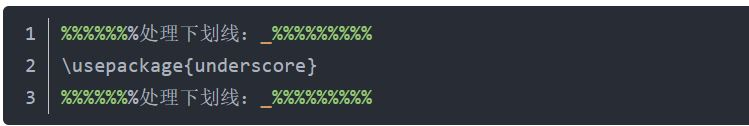
\includegraphics[width=.8\linewidth]{a.JPG}
  \caption{下划线处理.}
  \label{fig:boat1}
\end{figure}
2.插入图片
\begin{figure}
  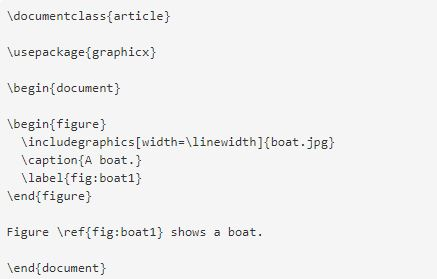
\includegraphics[width=.8\linewidth]{model.JPG}
  \caption{插入图片}
  \label{fig:boat1}
\end{figure}

$\#$的输入方法:
\subsection{ubuntu}
1.vim编辑器插入模式时左下角没有显示INSERT,而且退格键用不了。\\
解决方法:修改/etc/vim/vimrc.tiny 文件,将set compatible 设置成set nocompatible .这是因为有时候系统会默认vim兼容vi,所以使用vi的命令;/etc/vim/vimrc.tiny 文件加一行set backspace=indent,eol,start \\
打开文件或文件夹:xdg-open Ibex\\
2.编译\\
2.1 .cpp文件和makefile在同一文件夹下:\\
可直接用make命令编译(编译后生成可执行文件,只有重新修改了才能再次编译):\\
\begin{figure}
  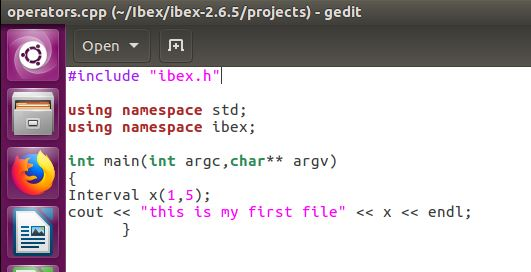
\includegraphics[width=.8\linewidth]{chengxu1.JPG}
  \caption{operators.cpp}
  \label{fig:boat1}
\end{figure}

\begin{figure}
  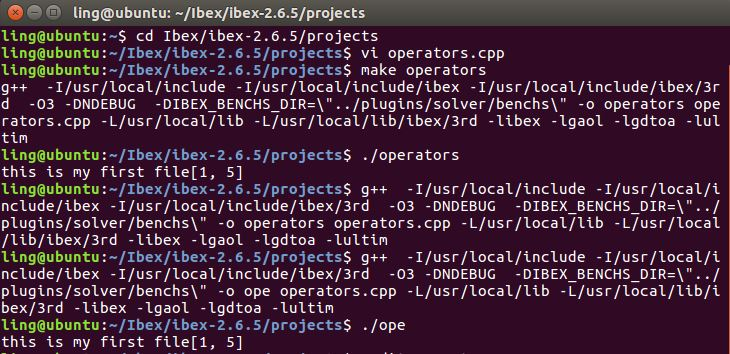
\includegraphics[width=.8\linewidth]{make1.JPG}
  \caption{make}
  \label{fig:boat1}
\end{figure}
2.2.cpp文件和makefile不在同一文件夹下,g++编译operator.cpp:\\
g++  -I/usr/local/include -I/usr/local/include/ibex -I/usr/local/include/ibex/3rd  -O3 -DNDEBUG  -DIBEX_BENCHS_DIR=\"../plugins/solver/benchs\" -o ope operator.cpp -L/usr/local/lib -L/usr/local/
lib/ibex/3rd -libex -lgaol -lgdtoa -lultim\\
它们二者都是把.cpp编译成可执行的文件,执行文件得到结果:\\
./ope
2.3 makefile的作用就是提供头文件和静态库的路径等作用。没有makefile,这些目录也可以通过pkg-config找到,如图5-7。

\begin{figure}
  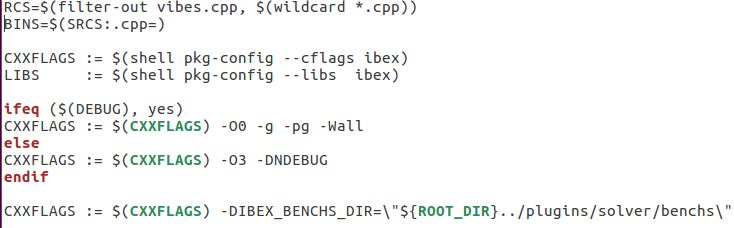
\includegraphics[width=.8\linewidth]{makefile.JPG}
  \caption{makefile introduce}
  \label{fig:boat1}
\end{figure}

\begin{figure}
  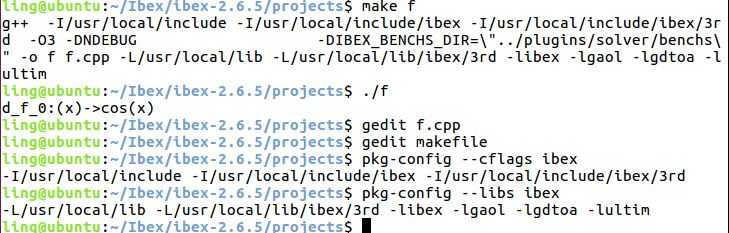
\includegraphics[width=.8\linewidth]{libs.JPG}
  \caption{libs directory}
  \label{fig:boat1}
\end{figure}
2.4 静态库是.a文件,链接.a静态库文件\\
gcc -o test dll_test.c -L  ./  SDKUseDll.a \\

说明: test是编译后的执行程序的名称,dll_test.c是源代码文件, -L  ./   是指包含.a文件包含的目录,我测试过程使用和源文件一样的当前目录,SDKUseDll.a为需要链接的静态库。便于测试,我是把.a文件需要的头文件和.a文件一并放入到.c的源代码文件的同一个目录下。\\
 如果把.a文件放入到源代码文件的lib子目录下,那么运行如下命令即可链接到: \\
  gcc -o test dll_test.c -L  ./lib  SDKUseDll.a\\
  
3.删除一个文件或文件夹:\\
rm -rf filename\\
4.pkg-config的基本用法:\\
找出头文件的路径 pkg-config --cflags ibex\\
找出静态库的路径 pkg-config --libs ibex\\
pkg-config --cflags --libs ibex\\
https://blog.csdn.net/zhoujiaxq/article/details/25972859\\
5.c++语法\\
int main(int argc,char** argv)  argc是返回参数的个数,argv表示具体返回的参数。\\
定义数组时一定要先定义数组类型,一般为double类型
同时输出多个变量: cout << a << "," << b << endl;
数组元素表示:a[2]和a(2)是不一样的,a[2]是第三个元素,而a(2)是第二个元素。
6.VIBes
VIBes是一个开源科学可视化系统,旨在为使用区间方法的人提供一种简单的方法来显示结果(boxes,subpaving),而无需担心图形用户界面编程。它提供了可从多种编程语言访问的绘图功能,而无需复杂的安装和库依赖性。VIBes由可视化程序和用于流行编程语言的应用程序编程接口组成(目前C ++和MATLAB,计划更多)。它专为任何项目中的即时设置而设计,具有非常短的学习曲线,这使其成为教学实验室和教程的良好可视化工具。程序和VIB之间的通信通过命名管道或文件进行,并包含在人类可读的消息中。提供非常简单的绘图功能,和VIBes查看器功能导航图纸和导出图像。本文介绍了推动VIB设计的主要概念及其软件架构。提供了显示设置反转问题的结果和投影的3-D数据的显示的两个短程序,并且详细描述了未来的发展方向。\\
7.problems\\
1. const ExprNode $\&$  中间变量\\
8.编程实现了从x到f的映射,解决了上次的问题。\\
\begin{figure}
  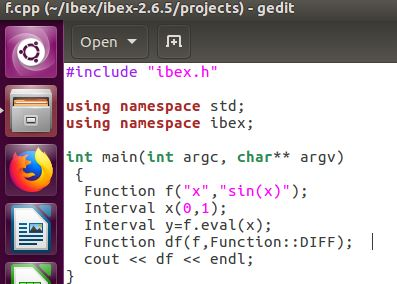
\includegraphics[width=.8\linewidth]{eval.JPG}
  \caption{f(x)}
  \label{fig:boat1}
\end{figure}

\begin{figure}
  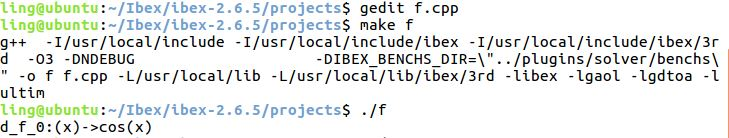
\includegraphics[width=.8\linewidth]{make2.JPG}
  \caption{f(x)}
  \label{fig:boat1}
\end{figure}
总结:/Ibex/ibex-2.6.5/projects :operators.cpp f.cpp  fun.cpp对应\\
/Tutorial/function/Functions with vector arguments\\
\subsection{applied interval analysis }
图书馆wos,EI搜索入口:\\
图书馆主页~电子资源数据库~检索工具\\
1.Constrained Wine Blending\\
Moore and Griffin have shown that aroma concentrations of a wine blending satisfy linear constraints.However, several other requirements lead to nonlinear constraints.\\

In this article, we present a mathematical modeling of the wine assemblage
problem. The problem is modeled by a mixed (discrete and continuous) nonlinear
program. We transform it into a non-linear (pure) continuous CSP handled
by a rigorous interval Branch and Bound (B $\&$ B). We have built a constrained
optimization model for minimizing in each target wine the gap between desired
aromatic concentrations and obtained concentrations, while taking into account
the minimal transfer disjunctive constraint. Absolute value and max operators
have been removed from the obtained system.\\
\section{2018.9.7}
\subsection{latex}
1.文本环境:https://blog.csdn.net/lishoubox/article/details/7295947\\
1.Constrained Wine Blending\\
概要:用Ibex(Interval based explorer)去优化葡萄酒混合物的芳香品质.(软件工具Kallosmé)\\
文章思路:(建模)确定变量~约束条件~目标函数   (优化)用Ibex工具求解\\
介绍了一些工具但是没有给出如何实现具体解决问题的过程。\\
1.1 在约束条件下的全局优化 \\
\begin{figure}
  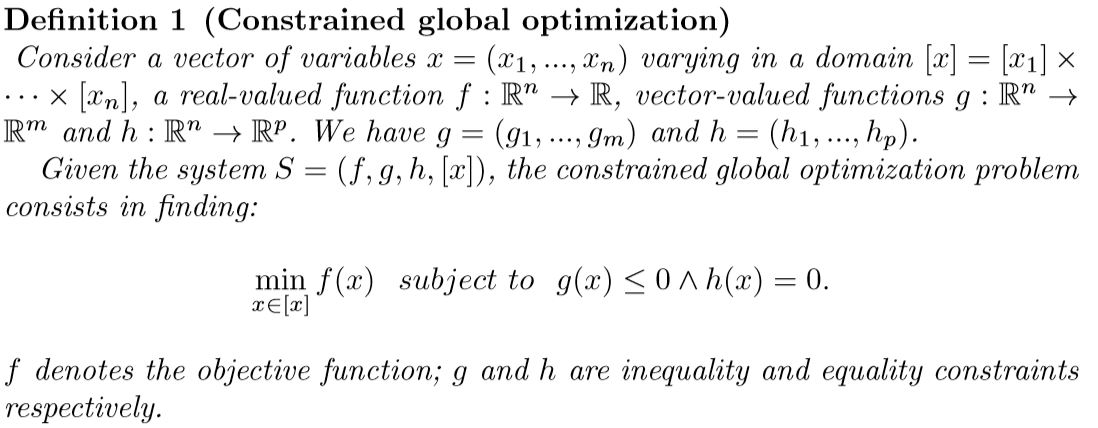
\includegraphics[width=.8\linewidth]{globelop.JPG}
  \caption{globel optimization}
  \label{fig:boat1}
\end{figure}

\subsection{线性规划}
在命令行逐行输入很不方便,而且无法保存命令。拟在Pycharm环境下利用pandas,pulp等解决线性规划问题\\
题一:\\
变量x,y,求出\\
\centerline{$z=4x+3y$}
的最大值,条件:\\
\begin{center}
$x\geq0$\\
$y\geq2$\\
$2y\geq25-x$\\
$4y\geq2x-8$\\
$y\geq2x-5$\\
\end{center}
在pycharm新建工程,工程下新建文件,选择类型为python,保存为lala.py后运行生成\\
运行结果:\\
\begin{figure}
  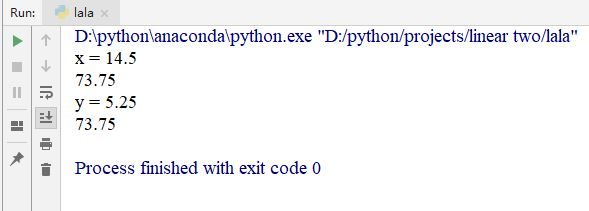
\includegraphics[width=.8\linewidth]{lala.JPG}
  \caption{linear programming}
  \label{fig:boat1}
\end{figure}
题二(如图13):
\begin{figure}
  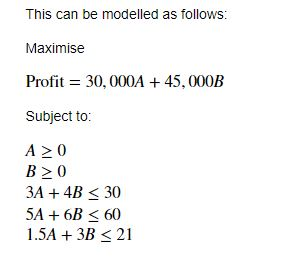
\includegraphics[width=.8\linewidth]{resourcepro.JPG}
  \caption{linear programming}
  \label{fig:boat1}
\end{figure}
文件为resource.py,由于pycharm环境不支持Magic函数,所以源程序第三行$\%$matplotlib inline显示出错\\
解决方法:换成from skimage import data,并在最后一行加上pilot.show()\\
运行结果:\\
\begin{figure}
  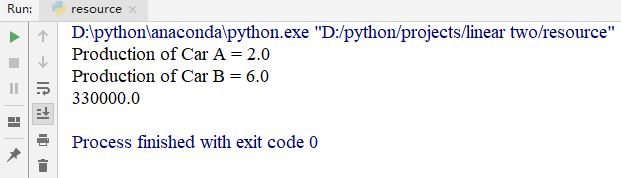
\includegraphics[width=.8\linewidth]{resource.JPG}
  \caption{linear programming}
  \label{fig:boat1}
\end{figure}
题三:\\
\begin{figure}
  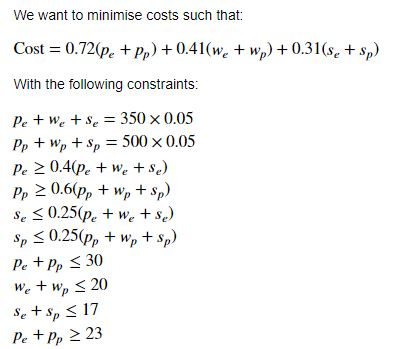
\includegraphics[width=.8\linewidth]{sausage.JPG}
  \caption{linear programming}
  \label{fig:boat1}
\end{figure}
运行结果:\\
\begin{figure}
  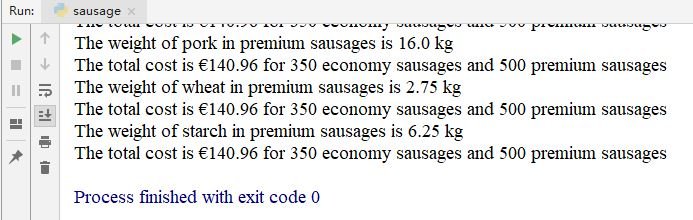
\includegraphics[width=.8\linewidth]{sausag.JPG}
  \caption{linear programming}
  \label{fig:boat1}
\end{figure}
题四:\\
\section{2018.9.9}
1./liuyan/pip/pip.ini
2.已经有anaconda,pycharm并配置好,pip install
\section{2018.9.10}
1.阅读Monnet的文章\\
基于结构约束条件下的无穷范数综合的全局优化问题,之前都是求一个控制器参数的唯一解,他的思路是利用区间分析方法求出多个符合要求的解,并筛选出最优解。\\
优点:可能得到一个传统方法得不到的更优解,结果更加可靠\\
缺点:在解决耦合约束条件下的问题效果不好;当自由变量的个数增加,算法复杂度呈现指数上升,求解难度增加。\\

\subsection{疑问}
1.$H_{\infty}$问题?\\
2. ACID算法\\
3.怎么从w到向量k的三个组成元素?\\
\subsection{Interval analysis(VIBes)}
VIBes是一个可视化系统,旨在为使用间隔方法的人提供一种显示结果(盒子,铺路)的方法,而无需担心GUI编程。它提供了可从许多编程语言访问的绘图功能,而无需复杂的安装和库依赖。VIBes的主要设计目标是跨平台,可从不同的编程语言中获得,设置简单,易于移植到新语言。\\

VIB由两部分组成:\\
1.VIBes应用程序,具有查看,注释和导出数字的功能\\
2.VIBes API,使您的程序能够与查看器进行通信,以便从C,C ++,Python,Matlab中绘制图形..\\

下载地址:https://github.com/ENSTABretagneRobotics/VIBES/releases\\

应用:\\
\begin{figure}
  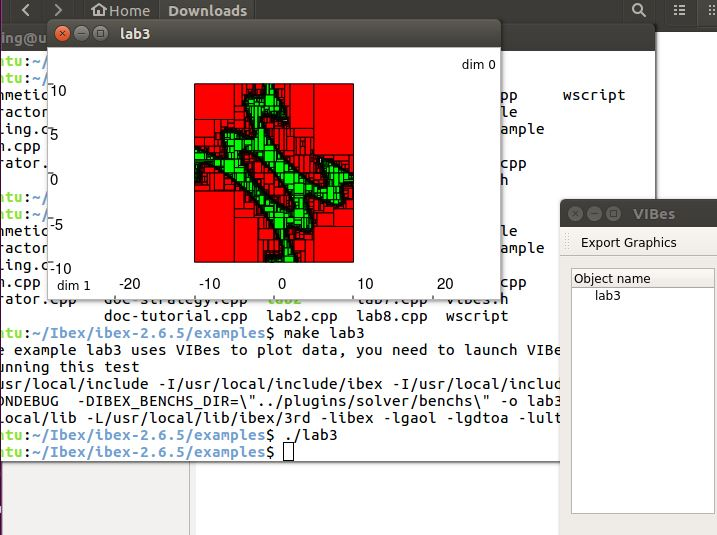
\includegraphics[width=.8\linewidth]{lab3.JPG}
  \caption{linear programming}
  \label{fig:boat1}
\end{figure}
\section{2018.9.11}
\subsection{线性规划}
1.题五:\\
利用pandas和pulp解决工厂调度问题:\\
\begin{figure}
  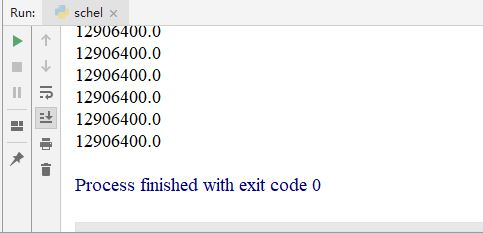
\includegraphics[width=.8\linewidth]{sch.JPG}
  \caption{linear programming}
  \label{fig:boat1}
\end{figure}
2.题六:\\
在题五的基础上引入新的附加方法:用0|1约束模拟条件语句,并运用到题五中考虑工厂的开或闭的月份,使结果更可靠.\\
\begin{figure}
  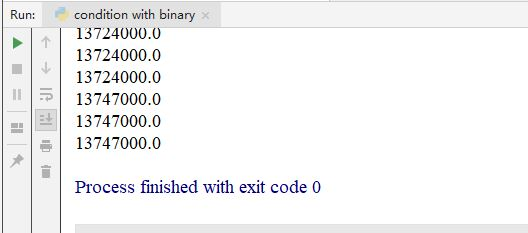
\includegraphics[width=.8\linewidth]{binary.JPG}
  \caption{linear programming}
  \label{fig:boat1}
\end{figure}
3.python命令行操作时,csv文件应该放置的路径https://blog.csdn.net/u010084228/article/details/78110145\\
4.解决the system is running in low-graphics mode:\\
连上网络,更新系统即可:\\
在报错页面点击ctrl+alt+F1打开终端,输入命令 sudo apt-get update   sudo apt-get upgrade ,然后reboot就OK了。\\
\subsection{applied interval analysis}
1.Krawczyk contractor
\begin{figure}
  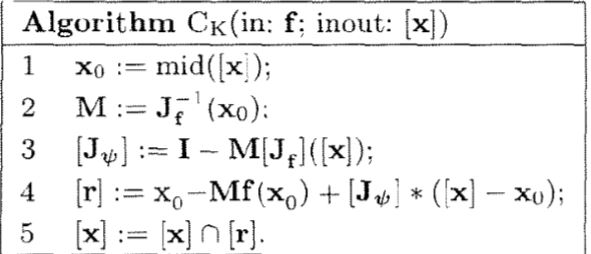
\includegraphics[width=.8\linewidth]{kra.JPG}
  \caption{linear programming}
  \label{fig:boat1}
\end{figure}

\end{document}


